\documentclass[12pt]{article}
\usepackage[margin=1in]{geometry} 
\usepackage{amsmath}
\usepackage{amssymb}
\usepackage{siunitx}
\usepackage{float}
\usepackage{tikz}
\def\checkmark{\tikz\fill[scale=0.4](0,.35) -- (.25,0) -- (1,.7) -- (.25,.15) -- cycle;} 
\usepackage{url}
\usepackage[siunitx,american,RPvoltages]{circuitikz}
\ctikzset{capacitors/scale=0.7}
\ctikzset{diodes/scale=0.7}
\usepackage{tabularx}
\newcolumntype{C}{>{\centering\arraybackslash}X}
\renewcommand\tabularxcolumn[1]{m{#1}}% for vertical centering text in X column
\usepackage{tabu}
\usepackage[spanish,es-tabla,activeacute]{babel}
\usepackage{babelbib}
\usepackage{booktabs}
\usepackage{pgfplots}
\usepackage{hyperref}
\hypersetup{colorlinks = true,
            linkcolor = black,
            urlcolor  = blue,
            citecolor = blue,
            anchorcolor = blue}
\usepgfplotslibrary{units, fillbetween} 
\pgfplotsset{compat=1.16}
\usepackage{bm}
\usetikzlibrary{arrows, arrows.meta, shapes, 3d, perspective, positioning,mindmap,trees,backgrounds}
\renewcommand{\sin}{\sen} %change from sin to sen
\usepackage{bohr}
\setbohr{distribution-method = quantum,insert-missing = true}
\usepackage{elements}
\usepackage{verbatim}
\usepackage[edges]{forest}
\usepackage{etoolbox}
\usepackage{schemata}
\usepackage{appendix}
\usepackage{listings}

\definecolor{color_mate}{RGB}{255,255,128}
\definecolor{color_plas}{RGB}{255,128,255}
\definecolor{color_text}{RGB}{128,255,255}
\definecolor{color_petr}{RGB}{255,192,192}
\definecolor{color_made}{RGB}{192,255,192}
\definecolor{color_meta}{RGB}{192,192,255}
\newcommand\diagram[2]{\schema{\schemabox{#1}}{\schemabox{#2}}}

\definecolor{codegreen}{rgb}{0,0.6,0}
\definecolor{codegray}{rgb}{0.5,0.5,0.5}
\definecolor{codepurple}{rgb}{0.58,0,0.82}
\definecolor{backcolour}{rgb}{0.95,0.95,0.92}

\lstdefinestyle{mystyle}{
    backgroundcolor=\color{backcolour},   
    commentstyle=\color{codegreen},
    keywordstyle=\color{magenta},
    numberstyle=\tiny\color{codegray},
    stringstyle=\color{codepurple},
    basicstyle=\ttfamily\footnotesize,
    breakatwhitespace=false,         
    breaklines=true,                 
    captionpos=b,                    
    keepspaces=true,                 
    numbers=left,                    
    numbersep=5pt,                  
    showspaces=false,                
    showstringspaces=false,
    showtabs=false,                  
    tabsize=2
}

\lstset{style=mystyle}
\usepackage{amsmath}
\usepackage{tcolorbox}
\usepackage{amssymb}
\usepackage{amsthm}
\usepackage{lastpage}
\usepackage{fancyhdr}
\usepackage{accents}
\usepackage{siunitx}
\pagestyle{fancy}
\setlength{\headheight}{42pt}

\begin{document}

\lhead{Ingeniería en Mantenimiento Industrial \\ Escuela de Ingeniría Electromecánica \\ Tecnológico de Costa Rica} 
\rhead{Electricidad I \\ Tarea \#5  \\ Entrega: Semana 12} 
\cfoot{\thepage\ de \pageref{LastPage}}
\noindent Los circuitos RL y RC pueden ser resueltos con ecuaciones diferenciales de primer orden, las ecuaciones de este tipo pueden ser resueltas con los modeladores/simuladores gráficos de sistemas dinámicos como Simulink de MATLAB y Xcos de Scilab. 

\vspace{0.5cm}
\noindent Por ejemplo, el siguiente circuito RL en serie vemos que: 

\begin{minipage}{.5\textwidth}
    \begin{gather*}
        v = v_R + v_L \\[6pt]
        v = i\cdot R + L\cdot \frac{di}{dt} \\[6pt]
        L\cdot \frac{di}{dt} = v - i\cdot R \\[6pt]
        di = \frac{v - i\cdot R}{L} \cdot dt\\[6pt]
        i = \int \frac{v - i\cdot R}{L} \cdot dt
    \end{gather*}
\end{minipage}% This must go next to `\end{minipage}`
\begin{minipage}{.5\textwidth}
    \begin{center}
            \begin{circuitikz}[scale=1]
            \draw
                (0,0)
                    to[V, l=$v$]
                (0,3)
                    to[R,l=$R$,i>^=$i$,v=$v_R$]
                (4,3)
                    to[L,l=$L$,v=$v_L$]
                (4,0) -- (0,0)
            ;
            \draw[white](-1,-1) rectangle (6,4);
            \end{circuitikz}
    \end{center}
\end{minipage}

\vspace{0.5cm}
\noindent Esta última ecuación se puede solucionar gráficamente usando Xcos, de la siguiente manera: 
\begin{center}
    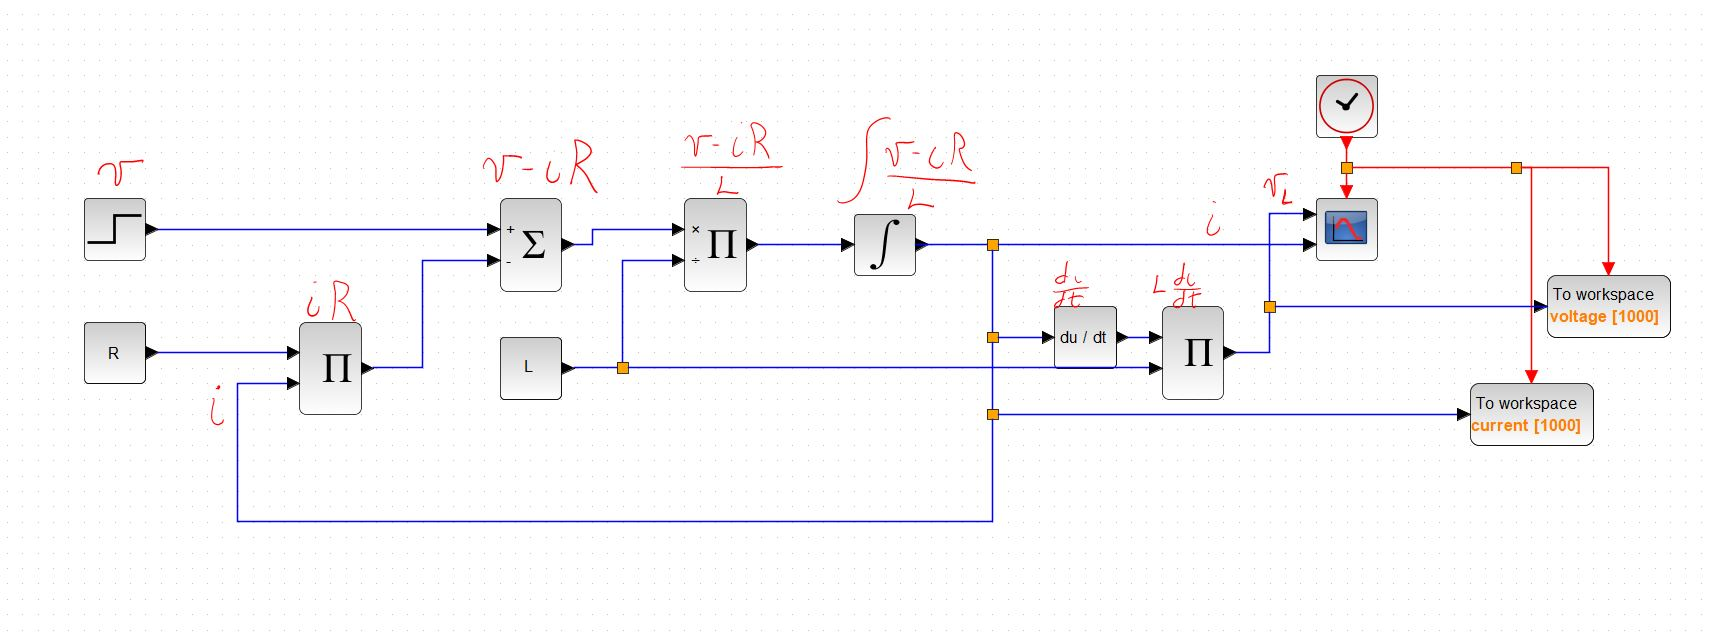
\includegraphics[width = \textwidth]{fig/RL_xcos.JPG}
\end{center}

\noindent\textbf{Instrucciones:}
\begin{itemize}
    \item Se proporciona un ejemplo funcional del circuito RL que incluye los scripts necesarios para comparar el resultado obtenido en Xcos con un resultado obtenido en LTSpice. Se debe partir de estos archivos y hacer las modificaciones correspondientes. 
    \item Se incluye un vídeo explicativo, se recomienda verlo antes de leer las siguientes instrucciones
    \item Usando Xcos, realice una solución análoga a la realizada por el instructor pero para un circuito RC en serie con $R=\SI{0.2}{\ohm}$ y $C=\SI{20}{\milli\farad}$. Incluya su solución en el informe de la tarea, debe ser similar a lo incluido al inicio de este documento 
    \item Excite el circuito usando una fuente $v=u(t-0.1)$ y obtenga los datos de corriente y voltaje del capacitor, guardelos en el espacio de trabajo tal como se muestra en el ejemplo proporcionado
    \item Realice una simulación en LTSpice del mismo circuito RC serie y guarde los datos de corriente y voltaje del capacitor en un archivo txt separado por tabs.
    \item Edite los scripts (.sce) de inicialización y de postprocesamiento de forma que se adapten a su nueva solución para el circuito RC en serie, documente el procedimiento usando comentarios que inicien con //
    \item Compare las gráficas de corriente y voltaje, incluya las comparaciones en el informe de la tarea
    \item Suba al TecDigital. Cualquier entrega tardía se califica por debajo de 70. 
\end{itemize}
\end{document}